\section{Evaluation}

\subsection{Data set}

Our dataset is the set called \textit{ANN\_IFT1M}\footnote{\url{http://corpus-texmex.irisa.fr/}}. Which is a set of 1,000,000 vectors with dimensionality 128. Vectors are stored as raw little endians. This dataset is created especially for measurements of the approximate nearest neighbour searches.

\subsection{Metrics}

\paragraph{Recall} Recall in information retrieval is the fraction of the data that are relevant to the query that are successfully retrieved.
\paragraph{Precision} Precision is the fraction of retrieved data that are relevant to the query.
\paragraph{Time} We have three different speed metrics to compare:

\begin{itemize}
  \item Construction time given in milliseconds.
  \item Insertion time given in nanoseconds.
  \item Query time given in seconds.
\end{itemize}

\paragraph{Memory consumption} Total amount of memory needed to create data structure and query it. Given in megabytes and gigabytes.

\subsection{Benchmark}

For measuring our metrics we are using library called \textit{hayai}\footnote{\url{https://github.com/nickbruun/hayai}}, small C++ framework for writting benchmarks. It provides toolkit for measuring time, multiple runs and iterations.

\subsection{Test environment}

Experiments were conducted on Intel i5 Processor with 8GB of RAM in 64 bit operating system. Our main idea is to compare and evaluate results of the two LSH implementations - the c "covering" and classic one. To do so we first load all data set to our data structure. And then querying them 1500 times for random element.

Classic table is constructed with given parameters

\begin{itemize}
  \item dimension = 128
  \item samples = 32 (which denotes how many bits we are sampling)
  \item partitions = 64
\end{itemize}

Obviously the Covering table is also created with the same dimension parameter. Only difference is the radius parameter. Which is one of the most important test cases. We test it again radius of 2,3,4,5,6. Any higher values requires more superior hardware in terms of memory.

\subsection{Results}

\begin{figure}[h]
  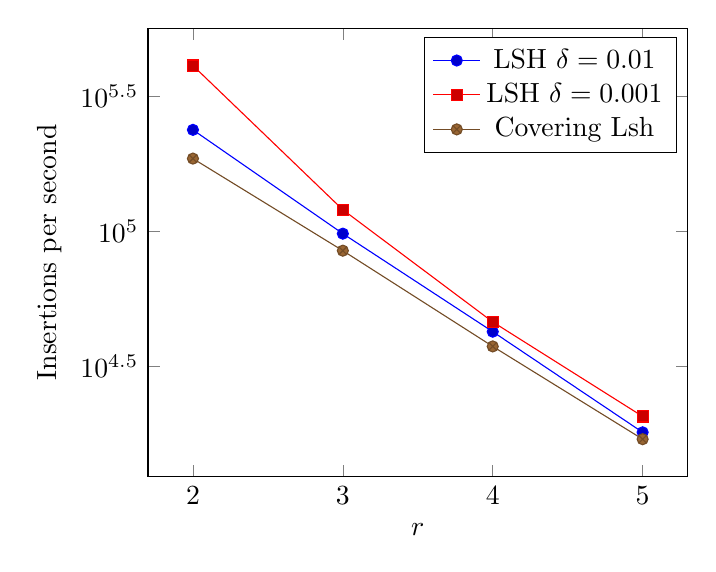
\begin{tikzpicture}
    \begin{semilogyaxis}[
      xlabel = {$r$},
      ylabel = {Insertions per second},
      xtick = data
    ]
      \addplot coordinates {
        (2, 237736.94)
        (3, 98187.51)
        (4, 42593.97)
        (5, 18074.10)
      };

      \addplot coordinates {
        (2, 411106.15)
        (3, 120359.67)
        (4, 46280.57)
        (5, 20693.81)
      };

      \addplot coordinates {
        (2, 186131.05)
        (3, 84934.71)
        (4, 37573.59)
        (5, 17047.07)
      };

      \legend{LSH $\delta = 0.01$, LSH $\delta = 0.001$, Covering Lsh}
    \end{semilogyaxis}
  \end{tikzpicture}
\end{figure}

\begin{figure}[h]
  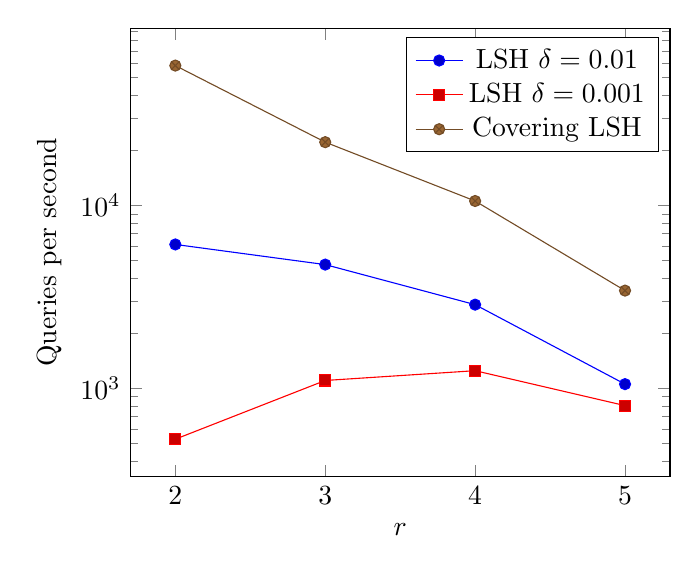
\begin{tikzpicture}
    \begin{semilogyaxis}[
      xlabel = {$r$},
      ylabel = {Queries per second},
      xtick = data
    ]
      \addplot coordinates {
        (2, 6118.88)
        (3, 4747.76)
        (4, 2866.80)
        (5, 1053.48)
      };

      \addplot coordinates {
        (2, 526.67)
        (3, 1103.17)
        (4, 1247.75)
        (5, 803.80)
      };

      \addplot coordinates {
        (2, 58216.55)
        (3, 22187.94)
        (4, 10574.71)
        (5, 3421.63)
      };

      \legend{LSH $\delta = 0.01$, LSH $\delta = 0.001$, Covering LSH}
    \end{semilogyaxis}
  \end{tikzpicture}
\end{figure}

\begin{figure}[h]
  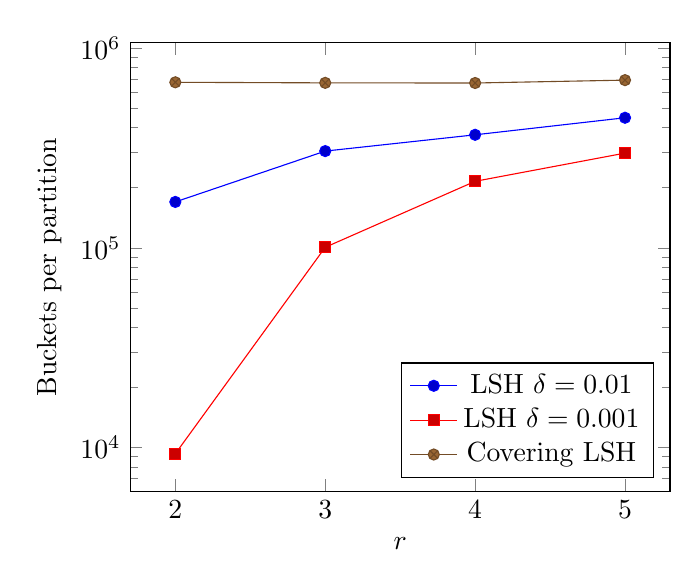
\begin{tikzpicture}
    \begin{semilogyaxis}[
      xlabel = {$r$},
      ylabel = {Buckets per partition},
      xtick = data,
      legend pos = south east
    ]
      \addplot coordinates {
        (2, 169815.43)
        (3, 305179.47)
        (4, 368261.81)
        (5, 448140.33)
      };

      \addplot coordinates {
        (2, 9310.57)
        (3, 100652.33)
        (4, 215357.87)
        (5, 298153.22)
      };

      \addplot coordinates {
        (2, 674554.00)
        (3, 670221.60)
        (4, 669083.68)
        (5, 691636.11)
      };

      \legend{LSH $\delta = 0.01$, LSH $\delta = 0.001$, Covering LSH}
    \end{semilogyaxis}
  \end{tikzpicture}
\end{figure}

\begin{figure}[h]
  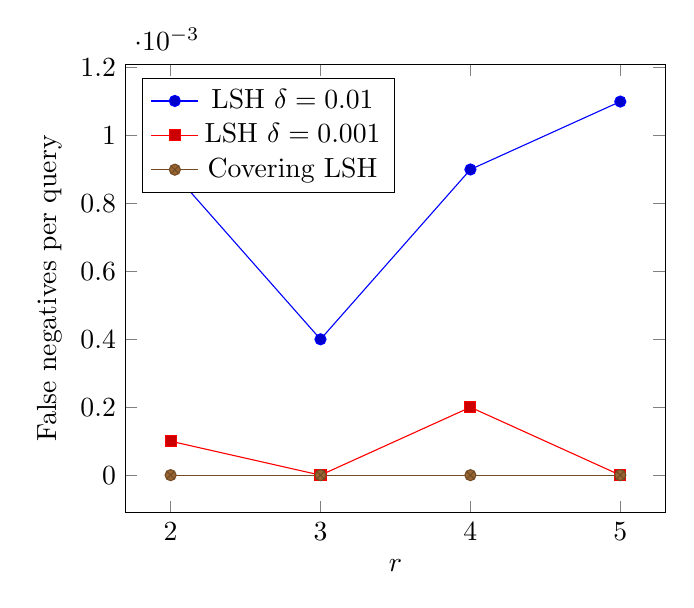
\begin{tikzpicture}
    \begin{axis}[
      xlabel = {$r$},
      ylabel = {False negatives per query},
      xtick = data,
      legend pos = north west
    ]
      \addplot coordinates {
        (2, 0.0009)
        (3, 0.0004)
        (4, 0.0009)
        (5, 0.0011)
      };

      \addplot coordinates {
        (2, 0.0001)
        (3, 0.0000)
        (4, 0.0002)
        (5, 0.0000)
      };

      \addplot coordinates {
        (2, 0.0000)
        (3, 0.0000)
        (4, 0.0000)
        (5, 0.0000)
      };

      \legend{LSH $\delta = 0.01$, LSH $\delta = 0.001$, Covering LSH}
    \end{axis}
  \end{tikzpicture}
\end{figure}
